%%%%%%%%%%%%%%%%%%%%%%%%
%
% $Author: Sadegh Naderi $
% $Datum: 2023-10-22  $
% $Shodrt Description: Bill of Materials for Keyword Spotting Project with Arduino Nano 33 BLE Sense $
%$Pfad: ML23-01-Keyword-Spotting-with-an-Arduino-Nano-33-BLE-Sense\report\Contents\en\BillofMaterials.tex $
% $Version: 5.0 $
% $Review by: Achal Shakywar and Sadegh Naderi $
% $Review date: 05.02.2024 $
%
%%%%%%%%%%%%%%%%%%%%%%%%


\chapter{Bill of Materials}
\label{chapter:BOM}

\section{Hardware Bill of Material}

The Table \ref{table:HardwareBOM} show the hardware requirements for this project. The Table \ref{table:OptionalHardwareBOM} shows the supplements which can be changed based on the preference of one. All of the materials on the list can be purchased through the \href{https://www.reichelt.de/}{reichelt} website. As can be seen from these tables, a laptop or desktop computer equipped with a USB port is essential as it serves as the primary programming environment. It is where programming, editing, and compiling of the embedded device's programs take place. The connection between the main computer and the embedded device is established via the USB port. It is worth noting that the main computer can run on various operating systems such as Windows, Linux, or macOS \cite{Warden:2019}.

\begin{table}[H]
	
	\begin{tabular}{m{3.0cm}|m{3.0cm}|m{1.7cm}|m{2cm}|m{1.5cm}}
		
		\hline
		
		\textbf{Hardware} & \textbf{Image} & \textbf{Quantity} & \textbf{Link} & \textbf{Price}\\
		
		\hline
		
		Board Arduino Nano 33 BLE Sense & \includegraphics[width=0.2\textwidth]{Images/ListofMaterials/ArduinoNano33BLESense} & 1 & \href{https://www.reichelt.de/arduino-nano-33-ble-sense-rev-2-nrf52840-ohne-header-ard-nano-33bs2-p336863.html?&trstct=pos_0&nbc=1}{reichelt}  &  36{,}60 \texteuro \\
		
		\hline
		
		GOOBAY 93922 USB 2.0 Cable, A male to micro B male, 0.60 m & \includegraphics[width=0.2\textwidth]{Images/ListofMaterials/USBCable} & 1 & \href{https://www.reichelt.de/usb-3-0-kabel-a-stecker-auf-a-stecker-0-5-m-goobay-95716-p249384.html}{reichelt}  &  2{,}30 \texteuro \\
		
		\hline
		
		FONTASTIC 262425 Powerbank, Li-Po, 10000 mAh, USB / USB-C & \includegraphics[width=0.2\textwidth]{Images/ListofMaterials/Powerbank} & 1 & \href{https://www.reichelt.de/powerbank-li-po-10000-mah-usb-usb-c-schwarz-fontastic-262425-p366911.html}{reichelt}  &  16{,}99 \texteuro \\
		
	\end{tabular}
	
	\caption {Hardware Bill of Materials}
	\label{table:HardwareBOM}
	
\end{table}

The Board Arduino Nano 33 BLE Sense is powered through a powerbank. Additionally, there's no need for an external microphone since the board comes equipped with a built-in microphone.



\begin{table}[H]
	
	\begin{tabular}{m{3.0cm}|m{3.0cm}|m{1.7cm}|m{2.3cm}|m{1.5cm}}
		
		\hline
		
		\textbf{Hardware} & \textbf{Image} & \textbf{Quantity} & \textbf{Link} & \textbf{Price}\\
		
		\hline
		
		ACER ABKEV.001 Laptop & 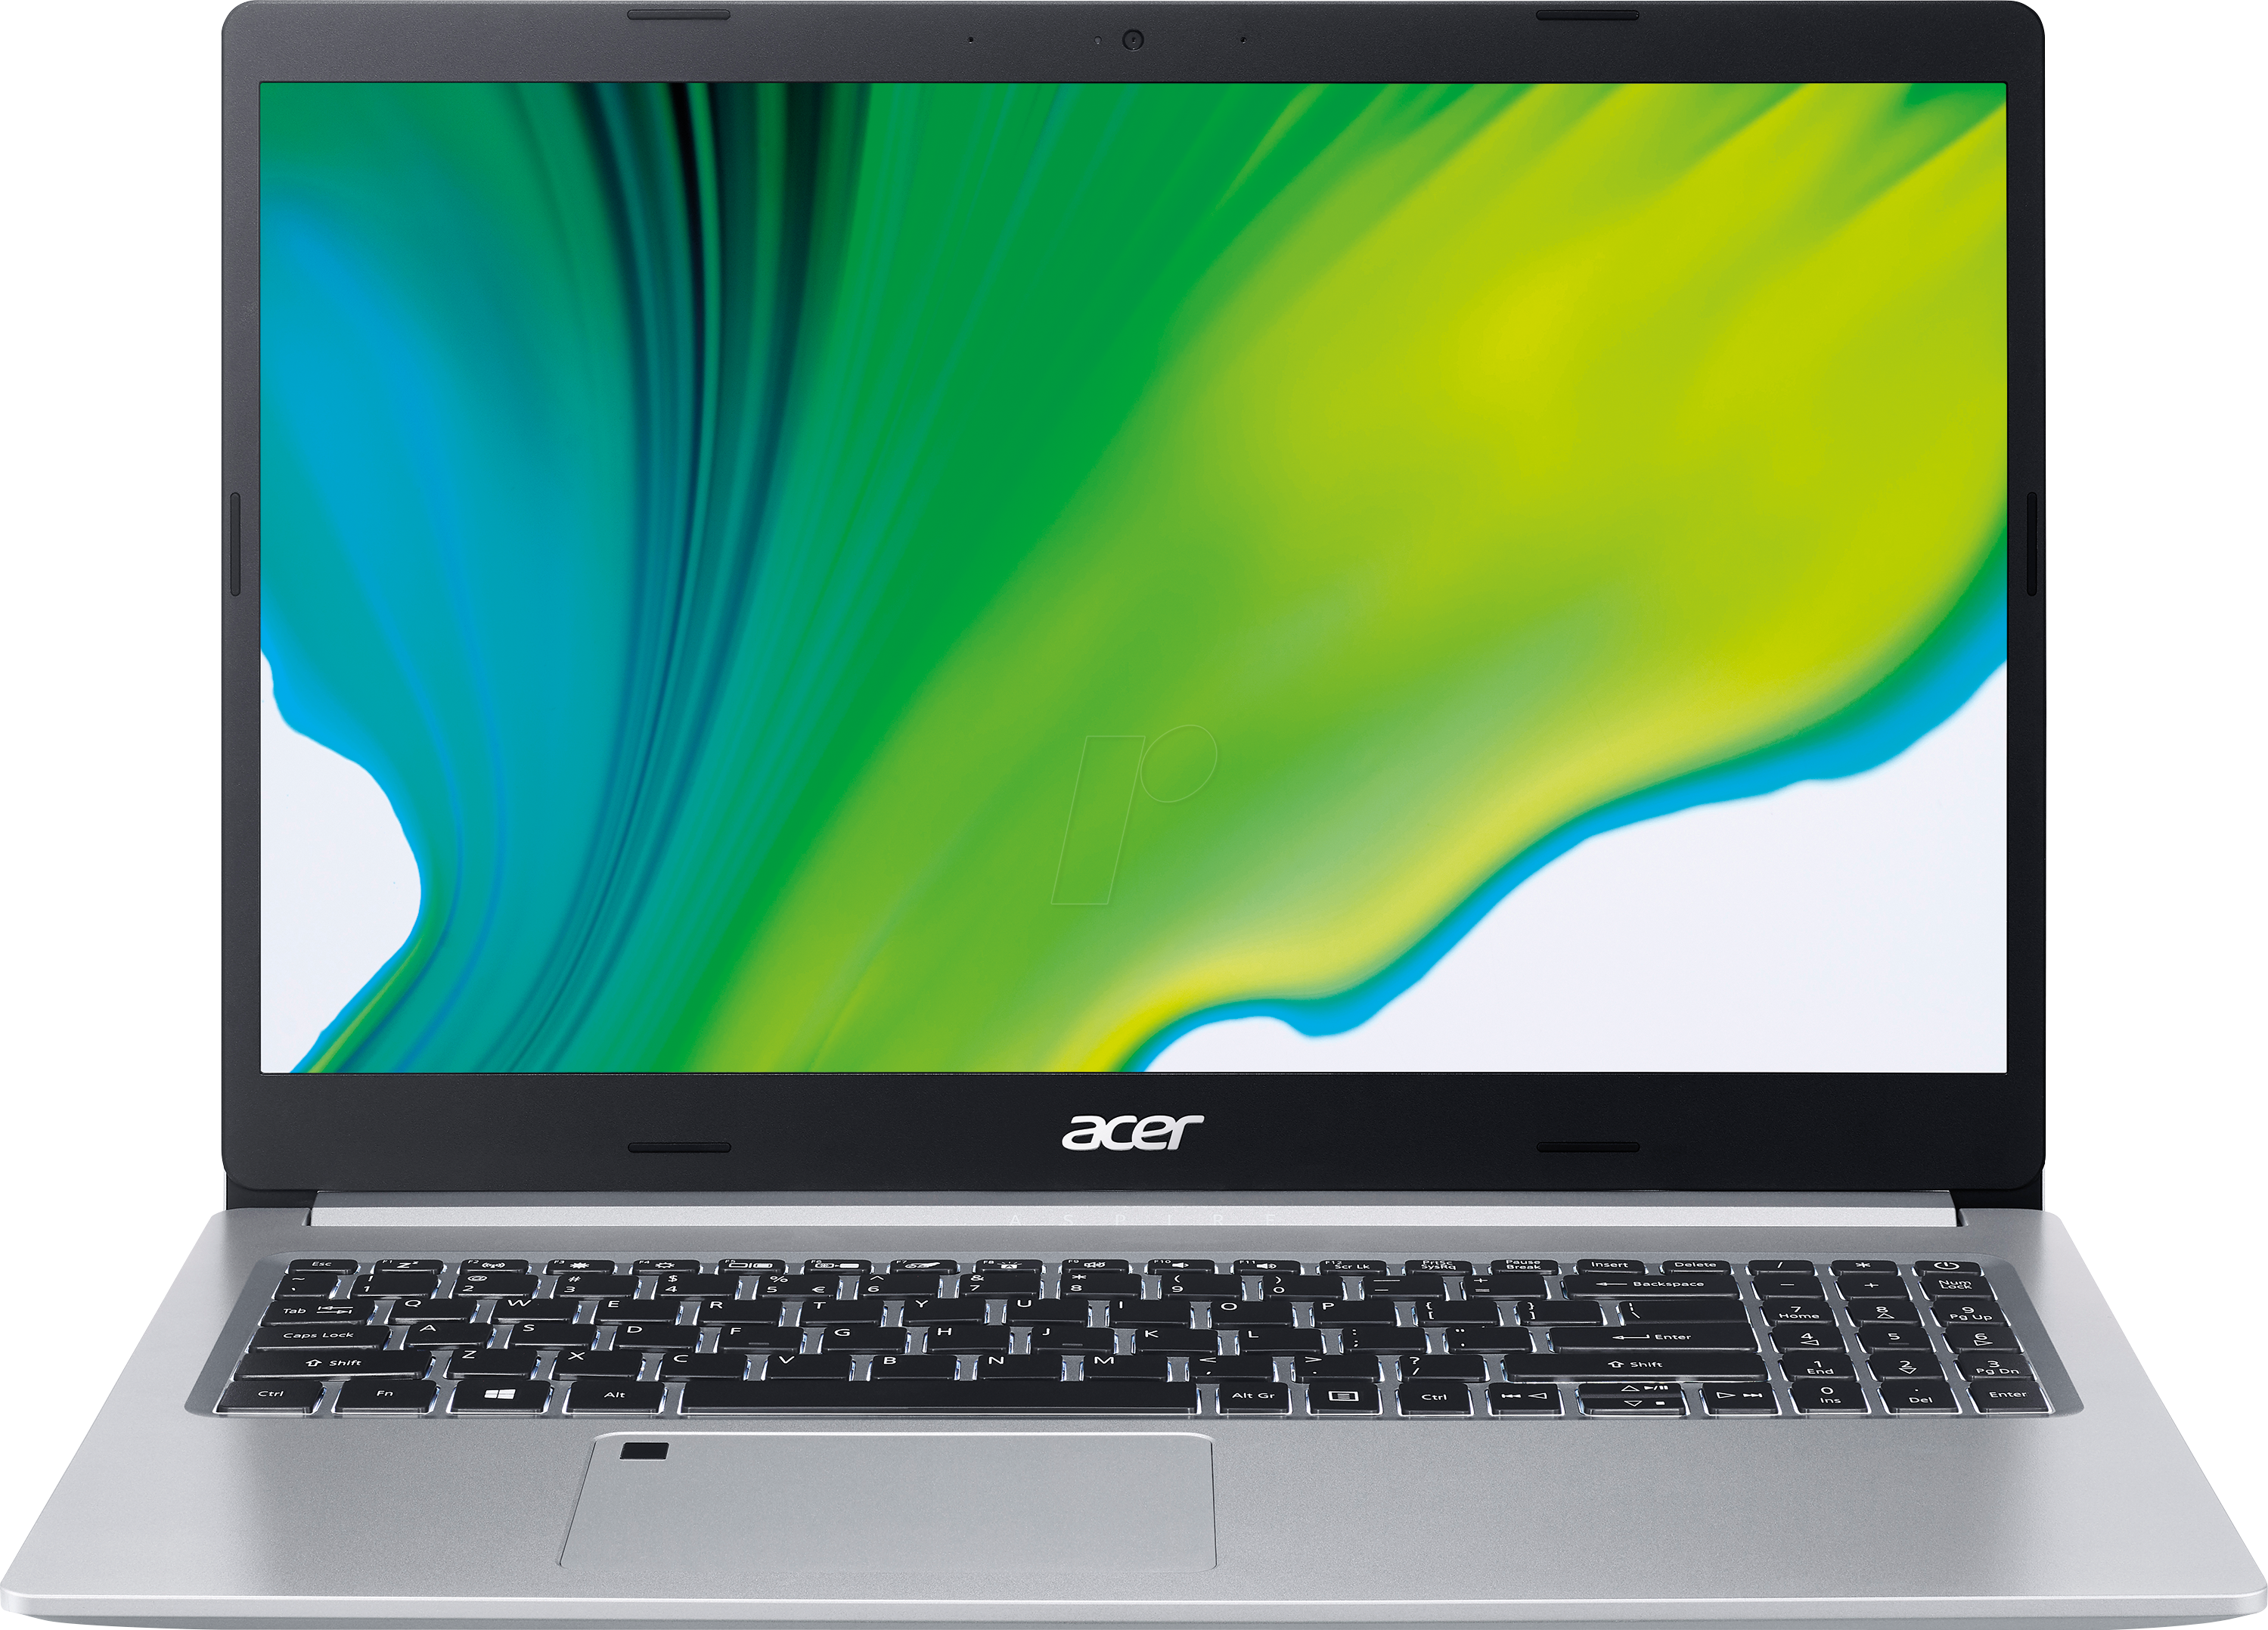
\includegraphics[width=0.2\textwidth]{Images/ListofMaterials/Laptop} & 1 & \href{https://www.reichelt.de/laptop-notebook-aspire-5-a515-45-r60r-windows-11-home-acer-abkev-001-p342777.html}{reichelt}  &  442{,}95 \texteuro \\
		
		\hline
		
		MANHATTAN 177658 Mouse & \includegraphics[width=0.2\textwidth]{Images/ListofMaterials/Mouse} & 1 & \href{https://www.reichelt.de/maus-mouse-kabel-usb-3-tasten-schwarz-manhattan-177658-p306883.html}{reichelt} & 3{,}95 \texteuro \\
		
	\end{tabular}
	
	\caption {Supplements}
	\label{table:OptionalHardwareBOM}
	
\end{table}


\section{Software Bill of Material (List of Packages and Tools)}

\subsection{Tools}

The table (Table \ref{table:ProgramBOM}) outlines the key specifications of the required programs for this project. It provides essential information including the software name, version, supported operating systems, license type, and a direct link for convenient access. The listed programs, Arduino IDE and PyCharm Community Edition, are integral to the development environment and cater to various operating systems, offering open-source licenses for accessibility and collaborative development. The provided links facilitate swift downloads, ensuring seamless integration into the project workflow.

\begin{table}[H]
	\centering
	\begin{tabular}{p{3cm}|p{1.5cm}|p{2cm}|p{2.5cm}|p{2cm}}
		\hline
		\textbf{Software} & \textbf{Version} & \textbf{Operating System} & \textbf{License} & \textbf{Link} \\
		\hline
		Arduino \ac{ide} & 2.2.1 & Windows, macOS, Linux & Open Source (GPL v2) & \href{https://www.arduino.cc/en/software}{Arduino IDE} \\
		\hline
		TensorFlow library for Arduino \ac{ide} & - & Windows, macOS, Linux & Open Source (Apache v2) & \href{https://github.com/tensorflow/tflite-micro-arduino-examples}{TensorFlow library} \\
		\hline
		PyCharm Community Edition & 2022.3.3 & Windows, macOS, Linux & Open Source (Apache 2.0) & \href{https://www.jetbrains.com/pycharm/}{PyCharm} \\
		\hline
		xxd for Windows & 1.11 & Windows & Open Source & \href{https://sourceforge.net/projects/xxd-for-windows/}{xxd for Windows} \\
		\hline
	\end{tabular}
	\caption{Required Tools}
	\label{table:ProgramBOM}
\end{table}

\subsubsection{TensorFlow}

TensorFlow is Google's open-source machine learning library, initially developed internally at Google and released to the public in 2015. It has since gained a substantial external community of contributors and is compatible with Linux, Windows, and macOS platforms. TensorFlow is the primary machine learning library used within Google, and its core code is consistent across both internal and public versions. While it provides a wide array of tools and optimizations for training and deploying models in the cloud, it was originally designed with a focus on desktop environments, prioritizing lower latency and added functionality, which might not be ideal for platforms with limited resources like Android and iPhone devices, where even a few megabytes added to an app's size can significantly impact downloads and user satisfaction. Building TensorFlow for these platforms typically increases the application size, and despite efforts, it remains relatively large, usually not shrinking below 2 MB even with optimization \cite{Warden:2019}.

\textbf{Installation Procedure}

The official TensorFlow Lite Micro library for Arduino is available in the tflite-micro-arduino-examples GitHub repository. To install the latest in-development version of this library, you can directly use the GitHub repository. This involves cloning the repository into the folder that contains libraries for the Arduino IDE. The location of this folder may vary by operating system, typically residing in \texttt{\textasciitilde/Arduino/libraries} on Linux, \texttt{\textasciitilde/Documents/Arduino/libraries/} on MacOS, and \texttt{My Documents\textbackslash Arduino\textbackslash Libraries} on Windows.

Once you are in that folder in the terminal, you can obtain the code using the \texttt{git} command line tool:

\begin{verbatim}
	git clone https://github.com/tensorflow/tflite-micro-arduino-examples Arduino_TensorFlowLite
\end{verbatim}

To update your cloned repository with the latest code, use the following terminal commands:

\begin{verbatim}
	cd Arduino_TensorFlowLite
	git pull
\end{verbatim}

\subsubsection{Arduino IDE}

Arduino IDE, short for Integrated Development Environment, is the official open-source software designed for editing, compiling, and uploading code onto Arduino modules \cite{Warden:2019}. Operating on the Java platform, it offers compatibility with a wide range of Arduino modules and supports both C and C++ programming languages. The Arduino Nano 33 BLE Sense employs this versatile IDE, which is the standard choice for programming all Arduino boards, offering the flexibility to work online and offline. Multiple software versions tailored to specific operating systems, such as macOS, Linux, and Windows, are available. Furthermore, the Arduino community provides an online coding platform that allows users to create and store their sketches in the cloud, and it consistently incorporates the latest IDE features and libraries while accommodating new Arduino boards. For the most recent software packages and information, you can access them through the following link: \url{https://www.arduino.cc/en/software}{arduino.cc/en/software}.

\subsubsection{xxd for Windows}

\texttt{xxd} is a hexdump utility that plays a key role in generating a hexadecimal representation of binary data, and in the context of this project, it is employed to facilitate the conversion process. The TFLite model, being a binary file, needs to be represented in a human-readable and manipulable format for certain operations, such as embedding it in C code. \texttt{xxd} provides the capability to create a hexdump of the TFLite model, making it easier to embed the model within C source code and ensuring compatibility with the project's requirements for model deployment and integration.

\textbf{Note}: Mac and Linux users don't need this requirement.

\subsubsection{PyCharm Community Edition Installation Guide:}

\begin{enumerate}
	\item \textbf{Download:}
	\begin{itemize}
		\item Go to the [PyCharm Community Edition download page](https://www.jetbrains.com/pycharm/download/).
		\item Download the installer for your operating system (Windows, macOS, or Linux).
	\end{itemize}
	
	\item \textbf{Installation on Windows:}
	\begin{itemize}
		\item Run the installer executable.
		\item Follow the installation wizard, selecting the default options unless you have specific preferences.
	\end{itemize}
	
	\item \textbf{Installation on macOS:}
	\begin{itemize}
		\item Open the downloaded disk image (.dmg) file.
		\item Drag the PyCharm icon to the Applications folder.
	\end{itemize}
	
	\item \textbf{Installation on Linux:}
	\begin{itemize}
		\item Extract the downloaded archive to a location of your choice.
		\item Navigate to the extracted folder and run the \texttt{bin/pycharm.sh} script.
	\end{itemize}
	
	\item \textbf{First Launch:}
	\begin{itemize}
		\item Launch PyCharm.
		\item Choose whether to import settings from a previous installation or start with default settings.
	\end{itemize}
	
	\item \textbf{Activation:}
	\begin{itemize}
		\item Activate PyCharm using a JetBrains account or continue with the free Community Edition.
	\end{itemize}
	
	\item \textbf{Usage:}
	\begin{itemize}
		\item Create a new Python project or open an existing one.
		\item Write and run your Python code in the PyCharm editor.
	\end{itemize}
\end{enumerate}

\subsubsection{Arduino IDE Installation Guide:}

For the installation guide refer to the Subsection \ref{subsection:SetupArduinoIDE}.


\subsubsection{License}

The licenses for the software in Table \ref{table:ProgramBOM} are critical in governing usage and distribution. Arduino IDE (v2.2.1) follows the GNU General Public License version 2 (GPLv2), ensuring open-source freedom for users. PyCharm Community Edition (v2022.3.3) is released under the Apache 2.0 license, providing users the liberty to utilize, modify, and distribute the Python development environment. These licenses foster collaboration and transparency, allowing developers to leverage and enhance these tools for diverse projects. Understanding these licenses is crucial for ethical and compliant use of these development resources.


\subsection{Packages}

The Table \ref{tab:pythonPackages} provides information on key Python packages used in the project, including their versions, licenses, and dependencies. The "Dependencies" column outlines the required dependencies for each package, indicating the version constraints where applicable. For a more detailed list of the packages, refer to the \href{run:../Code/KeywordSpotting/envRequirements/requirements.txt}{\texttt{requirements.txt}} file.


\begin{table}[h]
	\centering
	\begin{tabular}{l|l|l|l}
		\hline
		\textbf{Package} & \textbf{Version} & \textbf{License*} & \textbf{Dependencies} \\
		\hline
		Python & 2.9 & Open Source (PSF) & - \\
		\hline
		tensorflow & 2.15.0 & Open Source (Apache 2.0) & numpy (>=1.16.6) \\
		& & & gast (=0.3.3) \\
		& & & keras-preprocessing (=1.1.0) \\
		& & & keras-applications (=1.0.8) \\
		& & & tensorboard (=2.6.0) \\
		& & & termcolor (>=1.1.0) \\
		& & & wrapt (>=1.11.1) \\
		& & & absl-py (>=0.7.0) \\
		& & & grpcio (>=1.8.6) \\
		& & & astunparse (=1.6.3) \\
		& & & google-pasta (=0.2.0) \\
		& & & h5py (>=2.9.0) \\
		& & & opt-einsum (=3.3.0) \\
		& & & protobuf (>=3.12.2) \\
		\hline
		numpy & 1.26.2 & Open Source (BSD) & - \\
		\hline
		Matplotlib & 3.8.2 & Open Source (PSF) & cycler (>=0.10.0) \\
		& & & kiwisolver (>=1.0.1) \\
		& & & numpy (>=1.15) \\
		& & & Pillow (>=6.2.0) \\
		\hline
		Pandas & 2.1.4 & Open Source (BSD) & numpy (>=1.16.6) \\
		& & & python-dateutil (>=2.7.3) \\
		& & & pytz (>=2015.7) \\
		\hline
		pathlib & 2.9 & Open Source (PSF) & Python built-in \\
		\hline
		unittest & 2.9 & Open Source (PSF) & Python built-in \\
		\hline
		shutil & 2.9 & Open Source (PSF) & Python built-in \\
		\hline
	\end{tabular}
	\caption{Python packages and dependencies. \footnotesize{*PSF: Python Software Foundation, BSD: Berkeley Software Distribution}}
	\label{tab:pythonPackages}
\end{table}

\subsubsection{Short description}

\begin{itemize}
	\item \textbf{Python 3.9:}
	\begin{itemize}
		\item Python is the programming language in which your project is written. Python 3.9 is a stable and widely used version with numerous improvements and features compared to Python 2. Using the latest version is recommended for compatibility, security, and access to the latest language features.
	\end{itemize}
	
	\item \textbf{TensorFlow 2.15.0:}
	\begin{itemize}
		\item TensorFlow is a popular open-source machine learning library. In your project, it's likely used for developing and training machine learning models for keyword spotting. TensorFlow provides tools for building neural networks and processing audio data, which are essential for speech-related tasks.
		\begin{itemize}
			\item Note that \texttt{TensorFlow Lite} is used to facilitate the deployment of machine learning models on edge devices with limited resources. The framework provides tools like the TensorFlow Lite Converter, which optimizes models for memory-constrained devices, and supports quantization to reduce model size and improve execution speed on \ac{cpu}s \cite{Warden:2019}.
		\end{itemize}
	\end{itemize}
	
	\item \textbf{NumPy 1.26.2:}
	\begin{itemize}
		\item NumPy is a fundamental library for scientific computing in Python. It provides support for large, multi-dimensional arrays and matrices, along with mathematical functions to operate on these arrays. In your project, NumPy may be used for efficient handling and manipulation of numerical data, which is common in machine learning tasks.
	\end{itemize}
	
	\item \textbf{Matplotlib 3.8.2:}
	\begin{itemize}
		\item Matplotlib is a plotting library for creating visualizations in Python. In the context of your project, it may be used for visualizing data, training progress, or results. For instance, you might use Matplotlib to create graphs or spectrograms of audio data.
	\end{itemize}
	
	\item \textbf{unittest:}
	\begin{itemize}
		\item The \texttt{unittest} module is a testing framework that comes with Python. It provides a set of tools for constructing and running tests. It is inspired by the testing frameworks in other programming languages. The \texttt{unittest} module is part of the Python Standard Library, and its version is tied to the version of your Python interpreter. 
	\end{itemize}
	
	\item \textbf{pathlib:}
	\begin{itemize}
		\item The \texttt{pathlib} module provides an object-oriented interface for file system paths. It is used to handle paths more effectively and is introduced in Python 3.4 and later. The \texttt{pathlib} module is part of the Python Standard Library, and its version is tied to the version of your Python interpreter. 
	\end{itemize}
	
	\item \textbf{shutil:}
	\begin{itemize}
		\item The \texttt{shutil} module is a utility module for high-level file operations. It provides a higher-level interface compared to \texttt{os} module functions for file operations like copy, move, and delete. The \texttt{shutil} module is part of the Python Standard Library, and its version is tied to the version of your Python interpreter. 
	\end{itemize}
\end{itemize}


\subsubsection{Download and install}

To install Python 3.9, visit the official Python website at \url{https://www.python.org/downloads/release/python-390/}, download the installer for your operating system, and execute it. During installation, ensure to select the option to "Add Python 3.9.0 to PATH" for simplified command-line access. Follow the on-screen instructions to complete the installation. Verify the installation by opening a terminal or command prompt and entering the command; 

\begin{verbatim}
	python --version
\end{verbatim}

You should see "Python 3.9.0." 

Once Python is installed, you can proceed to install the required packages using the command line. Open a terminal or command prompt and navigate to your project directory. Then, execute the following command in the same directory that the \href{run:../Code/KeywordSpotting/envRequirements/requirements.txt}{\texttt{requirements.txt}} file exists:

\begin{verbatim}
	pip install -r requirements.txt
\end{verbatim}

This command reads the package requirements from the \href{run:../Code/KeywordSpotting/envRequirements/requirements.txt}{\texttt{requirements.txt}} file and installs them into your Python environment. Ensure that you have the \texttt{pip} tool installed and that it corresponds to the Python version you've installed. To install the packages without using the \href{run:../Code/KeywordSpotting/envRequirements/requirements.txt}{\texttt{requirements.txt}} file, one can execute the following command for the \texttt{tensorflow} and \texttt{numpy} packages for example:

\begin{verbatim}
	pip install tensorflow==2.15.0 numpy==1.26.2
\end{verbatim}

\subsubsection{Licenses}

The licenses for the packages in Table \ref{tab:pythonPackages} are vital in defining usage terms. Python follows the Python Software Foundation (PSF) license, granting freedom to use, modify, and distribute. TensorFlow employs the open-source Apache 2.0 license. NumPy, Pandas, and Matplotlib have open-source BSD and PSF licenses, fostering collaboration. The 'six' library, ensuring Python 2 and 3 compatibility, operates under the MIT license. Understanding these licenses is crucial for ethical and legal software use in development and data science.

\section{\href{run:../Code/KeywordSpotting/envRequirements/requirements.txt}{\texttt{requirements.txt}}}
\label{section:requirementsFile}

Utilizing Python requirements files is an effective method for managing Python modules. These files are straightforward text documents that store a compilation of the modules and packages essential for your project. By generating a requirements.txt file, you can effortlessly identify and install all the necessary modules manually.


\subsubsection{Benefits of Using \texttt{requirements.txt}:}

\begin{enumerate}
	\item Facilitates comprehensive tracking of Python modules and packages incorporated into your project.
	\item Streamlines the installation process of all required modules on any computer, eliminating the need for manual searches through online documentation or Python package repositories.
	\item Enables the seamless installation of dependencies on different computers, ensuring compatibility among them.
	\item Simplifies project sharing by allowing others to effortlessly install the specified Python modules listed in your \texttt{requirements.txt} file, enabling smooth project execution without complications.
	\item Offers a straightforward method for updating or adding Python modules to your project by simply modifying the \texttt{requirements.txt} file, eliminating the need to scour through your code for every reference to the outdated module.
\end{enumerate}

\subsection{Creating a \texttt{requirements.txt} File:}

Begin by navigating to your Python project directory and creating a new \texttt{.txt} document. Ensure it is named \texttt{requirements.txt} and save it in the same directory as your \texttt{.py} files for the project. At this point, there isn't much more to be done for creating a Python requirements file. However, we will delve into the manual installation of specific packages in the terminal.

Alternatively, you can generate a \texttt{requirements.txt} file directly from the command line using the following command:

\begin{verbatim}
	pip freeze > requirements.txt
\end{verbatim}

The \texttt{pip freeze} command outputs a list of all installed Python modules along with their respective versions.

\subsubsection{Adding Modules to Your \texttt{requirements.txt} File:}

The initial step involves opening the text document and inserting the names of the modules you intend to install. For instance, if you wish to incorporate the TensorFlow library into your project, type "tensorflow" on a new line along with the desired version. Consider the following example for your \texttt{requirements.txt} file:

\begin{verbatim}
	tensorflow==2.3.1
	uvicorn==0.12.2
	fastapi==0.63.0
\end{verbatim}

After including all the required modules, save the document.

\subsection{Installing Python Packages from a \texttt{requirements.txt} File}

\subsubsection{Utilizing the Package Manager Pip:}

To install packages from it, we will utilize the package manager \texttt{pip}. \texttt{Pip} is a versatile utility employed for the installation, upgrade, and uninstallation of Python packages. Additionally, it plays a role in managing Python virtual environments and more.

\subsubsection{Installing Python Packages from a \texttt{requirements.txt} File:}

To initiate \texttt{pip}, open a terminal or command prompt and navigate to your Python project directory. Once there, enter the following command:

\begin{verbatim}
	pip install -r requirements.txt
\end{verbatim}

This command installs all the modules specified in your Python requirements file into the project environment.

\textbf{Output:}

\begin{verbatim}
	Successfully installed absl-py-1.0.0 astunparse-1.6.3 ...
\end{verbatim}

\textbf{Note:}
It is advisable to set up a new environment before installing packages with your Python requirements file. If you need to remove a module, use the same command but replace "install" with "uninstall." Similarly, use "upgrade" instead of "install" to update previously installed Python packages. As mentioned earlier, employ the command \texttt{pip freeze} to generate a list of the Python modules installed in your environment.


\subsection{Maintaining a Python Requirements File}

\textbf{Step 1:} Output a list of outdated packages with \texttt{pip list --outdated}.

\textit{Output:}

\begin{verbatim}
	Package             Version  Latest  Type
	click               7.1.2    8.0.3   wheel
	fastapi             0.63.0   0.70.0  wheel
	gast                0.3.3    0.5.3   wheel
	h5py                2.10.0   3.6.0   wheel
	numpy               1.18.5   1.21.4  wheel
	pip                 20.0.2   21.3.1  wheel
	setuptools          44.0.0   59.5.0  wheel
	starlette           0.13.6   0.17.1  wheel
	tensorflow          2.3.1    2.7.0   wheel
	tensorflow-estimator 2.3.0    2.7.0   wheel
	uvicorn             0.12.2   0.15.0  wheel
\end{verbatim}

\textbf{Step 2:} Upgrade the required package with \texttt{pip install -U PackageName}. For example, updating \texttt{fastapi}:

\begin{verbatim}
	pip install -U fastapi
\end{verbatim}

\textit{Output:}

\begin{verbatim}
	Successfully installed anyio-3.4.0 fastapi-0.70.0 sniffio-1.2.0 starlette-0.16.0
\end{verbatim}

It is also possible to upgrade everything:

\begin{verbatim}
	pip install -U -r requirements.txt
\end{verbatim}

\textbf{Step 3:} Check to see if all tests pass.

\textbf{Step 4:} Run \texttt{pip freeze > requirements.txt} to update the Python requirements file.

\textbf{Step 5:} Run \texttt{git commit} and \texttt{git push} to the production branch.

Freezing all dependencies ensures predictable builds. To check for missing dependencies, use:

\begin{verbatim}
	python -m pip check
\end{verbatim}

\textit{Output:}

\begin{verbatim}
	No broken requirements found.
\end{verbatim}

\subsection{Creating a Python Requirements File After Development}

While it is possible to create it manually, it's good practice to use the \texttt{pipreqs} module. Install it with:

\begin{verbatim}
	pip install pipreqs
\end{verbatim}

Running \texttt{pipreqs} in the command line generates a file \texttt{requirements.txt} automatically:

\begin{verbatim}
	$ pipreqs /home/project/location
	Successfully saved requirements file in /home/project/location/requirements.txt
\end{verbatim}

\subsection{Why You Should Use a Python Requirements File}

Create a \texttt{requirements.txt} file when starting a new data science project. It's a best practice, particularly in the context of version control.

Using Python requirements files is among Python development best practices. It significantly reduces the need for managing and supervising different libraries. Managing library dependencies from one place makes it more convenient and faster compared to pasting a list of dependency paths into the command line.

GitHub provides automated vulnerability alerts for dependencies in your repository when you upload a \texttt{requirements.txt} with your code. It checks for conflicts and alerts the administrator if any are detected, and it can even resolve the vulnerabilities automatically.

\subsection{Contents of the \href{run:../Code/KeywordSpotting/envRequirements/requirements.txt}{\texttt{requirements.txt}} File}

In order to ensure a consistent and reproducible development environment, a set of Python dependencies and packages are specified in the \href{run:../Code/KeywordSpotting/envRequirements/requirements.txt}{\texttt{requirements.txt}} file. This file can be utilized to create an isolated environment using tools like Conda.

\begin{itemize}
	\item \texttt{absl-py=2.1.0=pypi\_0}: Google's Abseil library for Python, version 2.1.0 from the Python Package Index (PyPI).
	\item \texttt{astunparse=1.6.3=pypi\_0}: Library to unparse Python abstract syntax trees, version 1.6.3 from PyPI.
	\item \texttt{ca-certificates=2023.12.12=haa95532\_0}: SSL certificates required for secure connections.
	\item \texttt{cachetools=5.3.2=pypi\_0}: Generic caching library, version 5.3.2 from PyPI.
	\item \texttt{certifi=2024.2.2=pypi\_0}: Certificates for SSL/TLS, version 2024.2.2 from PyPI.
	\item \texttt{charset-normalizer=3.3.2=pypi\_0}: Library for URL encoding normalization, version 3.3.2 from PyPI.
	\item \texttt{flatbuffers=23.5.26=pypi\_0}: Library for efficient serialization of structured data, version 23.5.26 from PyPI.
	\item \texttt{gast=0.5.4=pypi\_0}: TensorFlow related package, version 0.5.4 from PyPI.
	\item \texttt{google-auth=2.27.0=pypi\_0}: Google Authentication Library, version 2.27.0 from PyPI.
	\item \texttt{google-auth-oauthlib=1.2.0=pypi\_0}: Library for integrating Google Authentication into OAuth2, version 1.2.0 from PyPI.
	\item \texttt{google-pasta=0.2.0=pypi\_0}: TensorFlow related package, version 0.2.0 from PyPI.
	\item \texttt{grpcio=1.60.1=pypi\_0}: High-performance RPC (Remote Procedure Call) framework, version 1.60.1 from PyPI.
	\item \texttt{h5py=3.10.0=pypi\_0}: HDF5 support for TensorFlow, version 3.10.0 from PyPI.
	\item \texttt{idna=3.6=pypi\_0}: Internationalized Domain Names in Applications (IDNA) library, version 3.6 from PyPI.
	\item \texttt{importlib-metadata=7.0.1=pypi\_0}: Library for accessing metadata for Python packages, version 7.0.1 from PyPI.
	\item \texttt{keras=2.15.0=pypi\_0}: High-level neural networks API, version 2.15.0 from PyPI.
	\item \texttt{libclang=16.0.6=pypi\_0}: Library for interacting with C, C++, and Objective-C code, version 16.0.6 from PyPI.
	\item \texttt{markdown=3.5.2=pypi\_0}: Markdown parsing library, version 3.5.2 from PyPI.
	\item \texttt{markupsafe=2.1.5=pypi\_0}: Library for XML/HTML markup safe string, version 2.1.5 from PyPI.
	\item \texttt{ml-dtypes=0.2.0=pypi\_0}: Machine learning data types library, version 0.2.0 from PyPI.
	\item \texttt{numpy=1.26.3=pypi\_0}: Fundamental package for scientific computing with Python, version 1.26.3 from PyPI.
	\item \texttt{oauthlib=3.2.2=pypi\_0}: OAuth library, version 3.2.2 from PyPI.
	\item \texttt{openssl=3.0.13=h2bbff1b\_0}: OpenSSL cryptographic library, version 3.0.13.
	\item \texttt{opt-einsum=3.3.0=pypi\_0}: Optimized contraction of multi-dimensional arrays, version 3.3.0 from PyPI.
	\item \texttt{packaging=23.2=pypi\_0}: Core utilities for Python packages, version 23.2 from PyPI.
	\item \texttt{pip=23.3.1=py39haa95532\_0}: Package installer for Python.
	\item \texttt{protobuf=4.23.4=pypi\_0}: Protocol Buffers, version 4.23.4 from PyPI.
	\item \texttt{pyasn1=0.5.1=pypi\_0}: ASN.1 types and codecs library, version 0.5.1 from PyPI.
	\item \texttt{pyasn1-modules=0.3.0=pypi\_0}: Collection of ASN.1 modules, version 0.3.0 from PyPI.
	\item \texttt{python=3.9.18=h1aa4202\_0}: Python programming language, version 3.9.18.
	\item \texttt{requests=2.31.0=pypi\_0}: HTTP library for Python, version 2.31.0 from PyPI.
	\item \texttt{requests-oauthlib=1.3.1=pypi\_0}: OAuthlib extension for Requests library, version 1.3.1 from PyPI.
	\item \texttt{rsa=4.9=pypi\_0}: RSA public key encryption algorithm, version 4.9 from PyPI.
	\item \texttt{setuptools=68.2.2=py39haa95532\_0}: Package development and distribution utilities.
	\item \texttt{six=1.16.0=pypi\_0}: Python 2 and 3 compatibility library, version 1.16.0 from PyPI.
	\item \texttt{sqlite=3.41.2=h2bbff1b\_0}: Self-contained, serverless, and zero-configuration SQL database engine, version 3.41.2.
	\item \texttt{tensorboard=2.15.1=pypi\_0}: TensorFlow's visualization toolkit, version 2.15.1 from PyPI.
	\item \texttt{tensorboard-data-server=0.7.2=pypi\_0}: TensorBoard data server, version 0.7.2 from PyPI.
	\item \texttt{tensorflow=2.15.0=pypi\_0}: Open-source machine learning library, version 2.15.0 from PyPI.
	\item \texttt{tensorflow-estimator=2.15.0=pypi\_0}: TensorFlow's high-level API for distributed training, version 2.15.0 from PyPI.
	\item \texttt{tensorflow-intel=2.15.0=pyp\_0}: TensorFlow with Intel optimizations, version 2.15.0 from PyPI.
	\item \texttt{tensorflow-io-gcs-filesystem=0.31.0=pypi\_0}: TensorFlow I/O library for Google Cloud Storage filesystem, version 0.31.0 from PyPI.
	\item \texttt{termcolor=2.4.0=pypi\_0}: ANSI color formatting for output in terminal, version 2.4.0 from PyPI.
	\item \texttt{typing-extensions=4.9.0=pypi\_0}: Type hints for Python, version 4.9.0 from PyPI.
	\item \texttt{tzdata=2023d=h04d1e81\_0}: Time zone database, version 2023d.
	\item \texttt{urllib3=2.2.0=pypi\_0}: HTTP library for Python, version 2.2.0 from PyPI.
	\item \texttt{vc=14.2=h21ff451\_1}: Compiler package for Microsoft Visual Studio, version 14.2.
	\item \texttt{vs2015\_runtime=14.27.29016=h5e58377\_2}: Visual Studio 2015 redistributable runtime, version 14.27.29016.
	\item \texttt{werkzeug=3.0.1=pypi\_0}: WSGI utility library for Python, version 3.0.1 from PyPI.
	\item \texttt{wheel=0.41.2=py39haa95532\_0}: Built-package format for Python.
	\item \texttt{wrapt=1.14.1=pypi\_0}: Function wrapper library for Python, version 1.14.1 from PyPI.
	\item \texttt{zipp=3.17.0=pypi\_0}: Backport of Python 3.10's zipapp module, version 3.17.0 from PyPI.
\end{itemize}

\subsection{Best Practices for Using a Python Requirements File}

\begin{itemize}
	\item Always use the command \texttt{pip freeze} to generate an up-to-date list of Python modules and packages installed in the virtual environment.
	\item Only list necessary Python modules and packages in \texttt{requirements.txt}.
	\item Save the \texttt{requirements.txt} in the project repository for easy installation by other developers.
	\item Use \texttt{pip install -r requirements.txt} to install all listed Python modules and packages.
	\item Keep \texttt{requirements.txt} up to date for the latest versions of Python modules and packages.
\end{itemize}


\section{\href{run:../Code/KeywordSpotting/envRequirements/environment.yml}{\texttt{environment.yml}} Conda Environment Configuration}
\label{section:CondaEnvConfig}

In this section, the contents of the \href{run:../Code/KeywordSpotting/envRequirements/environment.yml}{\texttt{environment.yml}} file are explained. To understand why and how it is produced, and see the use cases, see Chapter \ref{chapter:devEnv}.

\begin{verbatim}
	name: KeywordSpottingEnv
\end{verbatim}

This sets the name of the Conda environment to "KeywordSpottingEnv."

\begin{verbatim}
	channels:
	- defaults
\end{verbatim}

Specifies the channels from which to obtain packages. In this case, it includes the default Conda channel.

\begin{verbatim}
	dependencies:
	- ca-certificates=2023.12.12=haa95532_0
	- openssl=3.0.13=h2bbff1b_0
	- pip=23.3.1=py39haa95532_0
	- python=3.9.18=h1aa4202_0
	- setuptools=68.2.2=py39haa95532_0
	- sqlite=3.41.2=h2bbff1b_0
	- tzdata=2023d=h04d1e81_0
	- vc=14.2=h21ff451_1
	- vs2015_runtime=14.27.29016=h5e58377_2
	- wheel=0.41.2=py39haa95532_0
\end{verbatim}

Specifies the system-level dependencies for the Conda environment, including Python version, OpenSSL, SQLite, and other essential packages.

\begin{verbatim}
	- pip:
	- absl-py==2.1.0
	- astunparse==1.6.3
	- ...  % Other Python packages and their versions
\end{verbatim}

Specifies Python packages to be installed using \texttt{pip} within the Conda environment. It includes various TensorFlow-related packages and their specific versions.

\begin{verbatim}
	prefix: D:\Users\...\anaconda3\envs\KeywordSpottingEnv
\end{verbatim}

Specifies the path where the Conda environment will be created. 


